\documentclass{ieeeaccess}
\usepackage[UTF8]{ctex} 
\usepackage{cite}
\usepackage{amsmath,amssymb,amsfonts}

\usepackage{booktabs}
\usepackage{array}
\usepackage{multirow}
\usepackage{longtable}
\usepackage{rotating}
\usepackage[utf8]{inputenc} % allow utf-8 input
\usepackage[T1]{fontenc}    % use 8-bit T1 fonts


\usepackage{algorithmic}
\usepackage{subfigure}
\usepackage{graphicx}
\usepackage{textcomp}
\def\BibTeX{{\rm B\kern-.05em{\sc i\kern-.025em b}\kern-.08em
    T\kern-.1667em\lower.7ex\hbox{E}\kern-.125emX}}
\begin{document}
\history{Date of publication xxxx 00, 0000, date of current version xxxx 00, 0000.}
\doi{10.1109/ACCESS.2017.DOI}

\title{Preparation of Papers for IEEE ACCESS}
\author{\uppercase{Hao Li}\authorrefmark{1}, \IEEEmembership{Member, IEEE},
\uppercase{Second B. Author\authorrefmark{2}, and Third C. Author,
Jr}.\authorrefmark{3},
\IEEEmembership{Member, IEEE}}
\address[1]{Beijing University of chemical and technology, Beijing, 10029 China (e-mail: 2018040206@mail.buct.edu.cn)}
\address[2]{Department of Physics, Colorado State University, Fort Collins, 
CO 80523 USA (e-mail: author@lamar.colostate.edu)}
\address[3]{Electrical Engineering Department, University of Colorado, Boulder, CO 
80309 USA}
\tfootnote{This paragraph of the first footnote will contain support 
information, including sponsor and financial support acknowledgment. For 
example, ``This work was supported in part by the U.S. Department of 
Commerce under Grant BS123456.''}

\markboth
{Author \headeretal: Preparation of Papers for IEEE TRANSACTIONS and JOURNALS}
{Author \headeretal: Preparation of Papers for IEEE TRANSACTIONS and JOURNALS}

\corresp{Corresponding author: First A. Author (e-mail: author@ boulder.nist.gov).}

\begin{abstract}
blablabla
\end{abstract}

\begin{keywords}
U-Net, Biomedical image segmentation, Attention
\end{keywords}

\titlepgskip=-15pt

\maketitle

\section{Introduction}
\label{sec:introduction}
\PARstart{T}{his} document 

\section{Method}
\subsection{Network Architecture}
\begin{figure*}[htbp]
    \xdef\xfigwd{\textwidth}% 通栏浮动体,把它定义为 \textwidth
    \centering
    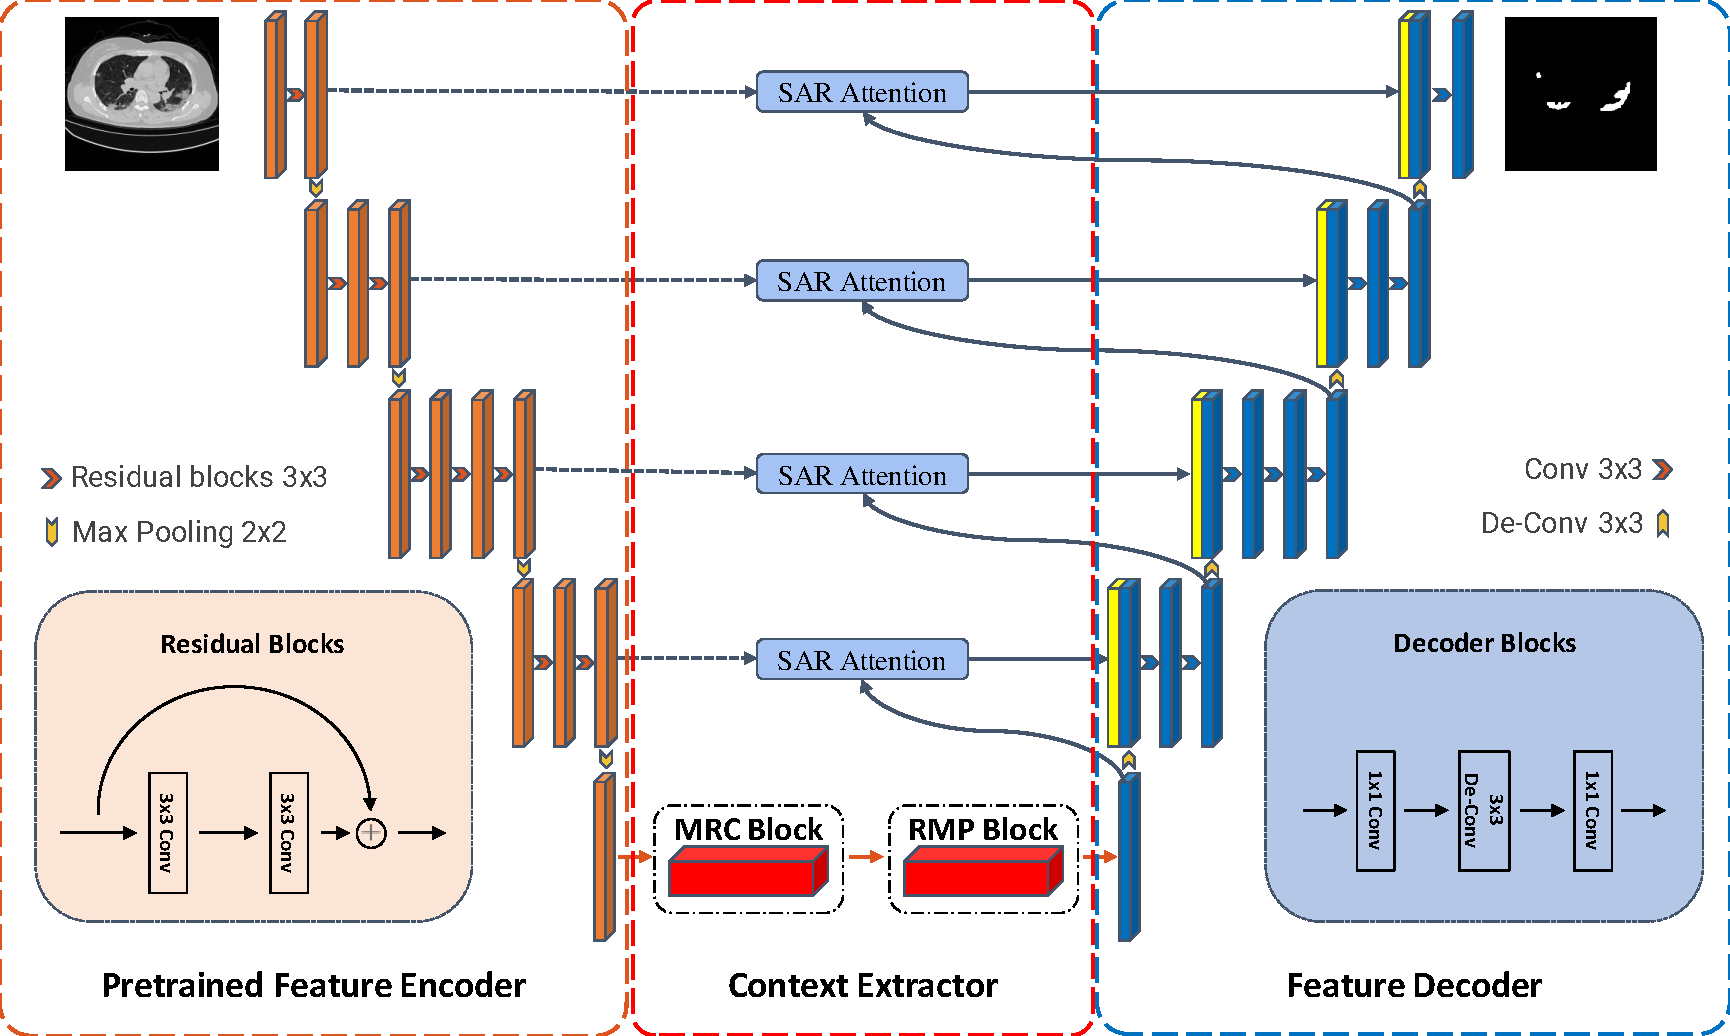
\includegraphics[width=0.9\textwidth]{figure/overview.pdf}
    \label{fig:overview}
    \caption{Illustration of our proposed network.}

\end{figure*}

\subsection{Bottleneck Modules}
在语义分割任务中,deep convolutional layers已经展现出其对提取图像特征的重要性。等人提出了CE-Net\cite{cenet},其在Bottleneck采用了DeepLab中的SPP-Block

\begin{table}[htbp]
  \vspace{-2mm}
  \begin{center}\small
  \label{param-table}
  \begin{tabular}{ccccccc}
    
  \toprule
  Backbone & Components & Params & Params size \\
  \midrule
    CE-Net & SAR & 135,571,137 & 517.16 \\
    ResU-Net & SAR+ASPP    & 92,573,377 & 353.14  \\
    ResU-Net & SAR+MRC+RMP & 94,669,505 & 361.14  \\
\bottomrule    
  \end{tabular}
  \caption{Memorize Cost Comparison With Different Methods In Bottleneck}
\end{center}
  %\vspace{-0.35cm}
  \vspace{-4mm}
\end{table}

\begin{figure*}[htbp]
    \xdef\xfigwd{\textwidth}% 通栏浮动体,把它定义为 \textwidth
    \centering
    \subfigure[Inception Module, also called DAC Block in CE-Net]
      {\centering
      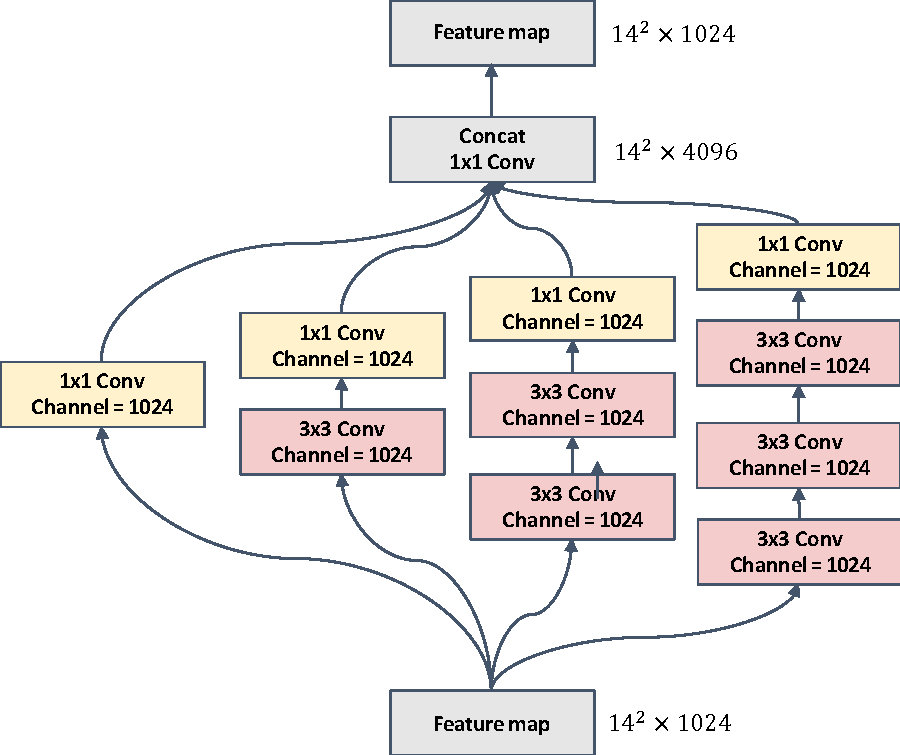
\includegraphics[width=0.35\textwidth]{figure/DAC_block.pdf}\label{dac_block}
      }
    \qquad
    \subfigure[MRC block]
      {\centering
      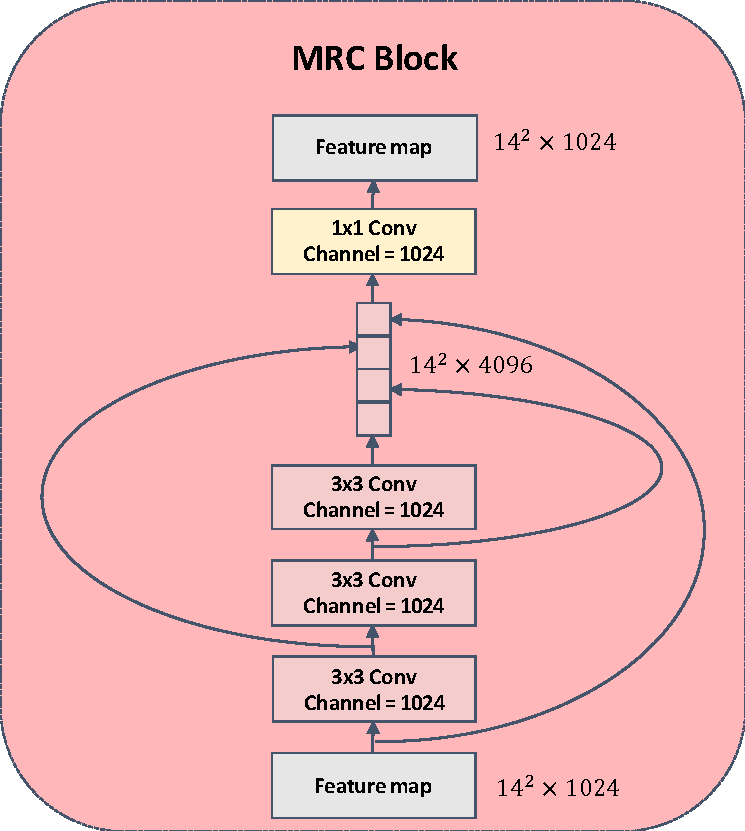
\includegraphics[width=0.35\textwidth]{figure/MRC_block.pdf}\label{mrc_block}
      }
    \caption{(\ref{dac_block}) is the illustration of DAC Block. (\ref{mrc_block}) is the illustration of MRC Block.}
    
\end{figure*}

\subsection{Attention Modules}
\begin{figure*}[htbp]
    \xdef\xfigwd{\textwidth}% 通栏浮动体,把它定义为 \textwidth
    \centering
    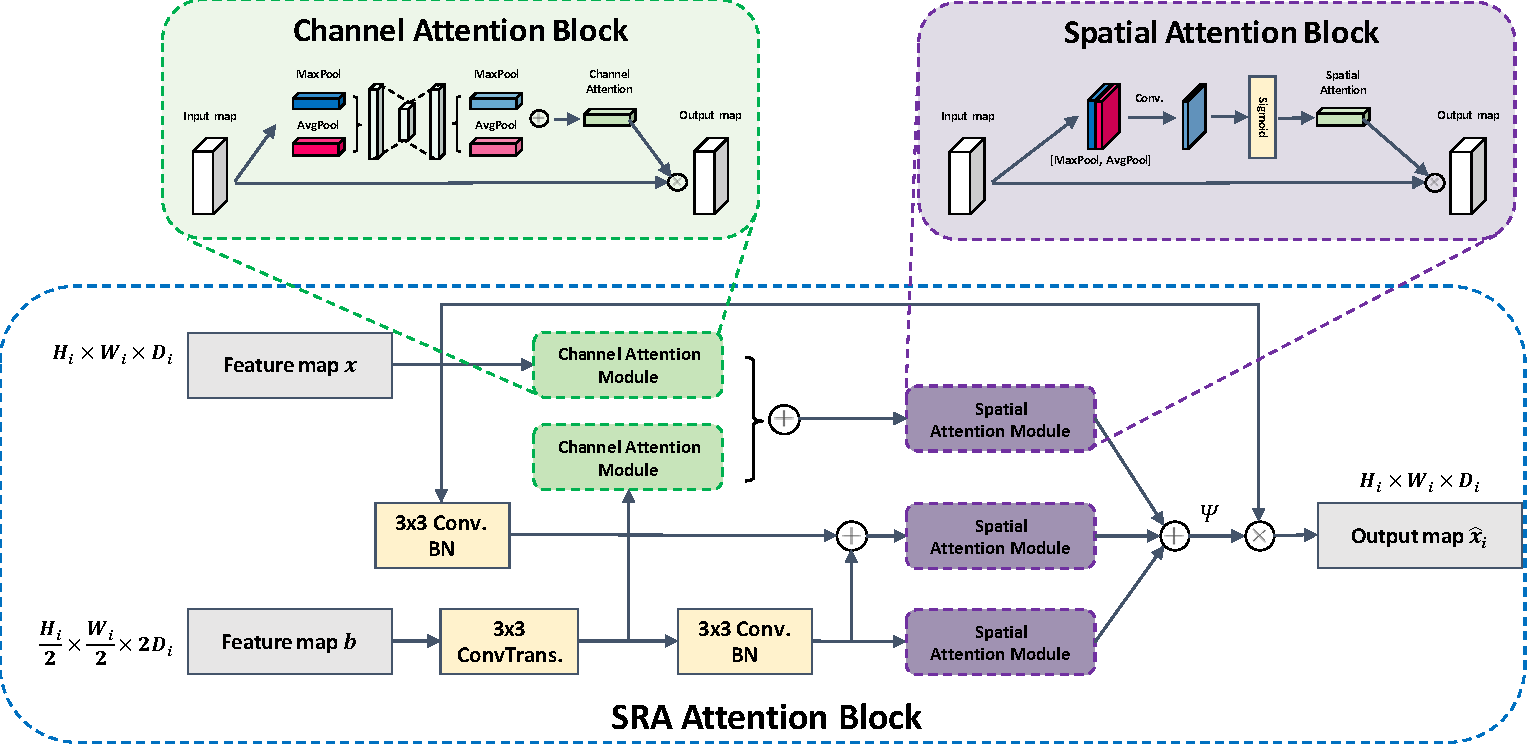
\includegraphics[width=0.9\textwidth]{figure/Attention.pdf}
    \label{fig:overview}
    \caption{Illustration of SRA Attention Block.}
\end{figure*}
\section{Experiments}
\subsection{Baseline and implementation}
We used a server equipped with an Intel Core i9-9980XE CPU @ 3.00GHz with 64GB RAM and 12GB of RTX2080Ti GPU for
our proposed networks training. The operating system of the sever is 64-bits Ubuntu 18.04. The structure of the network 
is implemented under the open source deep learning library Pytorch with VSCode implementation.

\subsection{Dataset}
For this study, we conduct our experiments on four differents segmentation tasks. 
Covering lesions/organs from most commonly used medical imaging modalities including microscopy, 
computed tomography (CT), and magnetic resonance imaging (MRI).  Table \ref{dataset-table} summarize those datasets in our study.

\begin{table}[htbp]
    \vspace{-2mm}
    \begin{center}\small
    \label{dataset-table}
    \begin{tabular}{ccccc}
      
    \toprule
    Dataset & Image & Input Size & Modality & Provider\\
    \midrule
    Cell & 30 & $512\times 512$  & EM      & ISBI 2012\cite{isbicell}   \\
    Liver    & 4,000 & $512\times 512$       & CT     & LiTS 2017\cite{liver}  \\
    DSB2018      & 670 & $256\times 256$      & EM      & Kaggle\cite{dsb2018} \\
    COVID19         & 1,800 & $630\times 630$     & CT     & Web\cite{covid19,covid19_2}  \\
  \bottomrule    
    \end{tabular}
    \caption{Summaey Of Biomedical Image Segmentation Datasets Used In Our Experiments}
  \end{center}
    %\vspace{-0.35cm}
    \vspace{-4mm}
\end{table}
  


\paragraph{Cell}
The datset is the segmentation of neuronal structures in electron microscopic recordings.
The dataset is provided by the EM segmentation challenge\cite{isbicell} that is started at ISBI 2012.
The data is a set of 30 images ($512\times 512$ pixels) from serial section transmission electron
microscopy of the Drosophila first instar larva ventral nerve cord (VNC). Each image comes with a corresponding fully annotated ground truth segmentation
map for cells (white) and membranes (black).

\paragraph{Liver}
Liver tumor Segmentation Challenge (LiTS)\cite{liver} contain 131 contrast-enhanced CT images provided by hospital around the world with \(512 \times 512\) resolution.
The ground truth segmentation provides two different labels: liver and lesion. For our experiments,
we only consider liver as positive class and others as negative class.


\paragraph{COVID19}
Dataset\cite{covid19} includes whole volumes and includes, therefore, both positive and negative slices 
(373 out of the total of 829 slices have been evaluated by a radiologist as positive and segmented). 
Dataset\cite{covid19_2} contains 20 CT scans of patients diagnosed with COVID-19 as well as segmentations of lungs and infections made by experts.
These volumes are converted and normalized in a similar way as above, meanwhile we resize the data to $512\times 512$.

\subsection{Evaluation metrics}
The experiments are implemented using the Pytorch framework. We use Adam optimizer\cite{Adam} as our
models' optimizer with a learning rate of 0.00001, batch size of 2. All of datasets are splitted into training set, validation set and test set with 
the ratio of 8:1:1 using sklearn library. To numerically evaluate, we use five widely adopted metrics, \(i.e.\),
the Dice similarity coefficient(Dice.), F1 score., Sensitivity(Sen.), Iou. and hausdorff distance(Hd)., the expressions of them are defined as follows:
\begin{align}
  \text { Sensitivity }=\frac{T P}{T P+F N}
\end{align}
\begin{align}
  \operatorname{DSC}(G, S)=\frac{2|G \cap S|}{|G|+|S|}
\end{align}
\begin{align}
  \operatorname{IOU}(G, S)=\frac{|G \cap S|}{|G| \cup|S|}
\end{align}
\begin{align}
  F_{1}=2 \cdot \frac{\text { precision } \cdot \text { recall }}{\text { precision }+\text { recall }}
\end{align}
\begin{align}
  h(G, S)=\max _{g \in G}\left\{\min _{c \in C}\|g-c\|\right\}
\end{align}
\subsection{Medical image Segmentation Results}
For comparsion, we use five origianl network FCN with 32s\cite{fcn}, U-Net\cite{unet}, U-Net++\cite{unet++} , CE-Net\cite{cenet} and U-Net with Attention Gate\cite{attentiongate}
to evaluate our proposaed method. 
\begin{figure*}[htbp]
  \begin{center}
  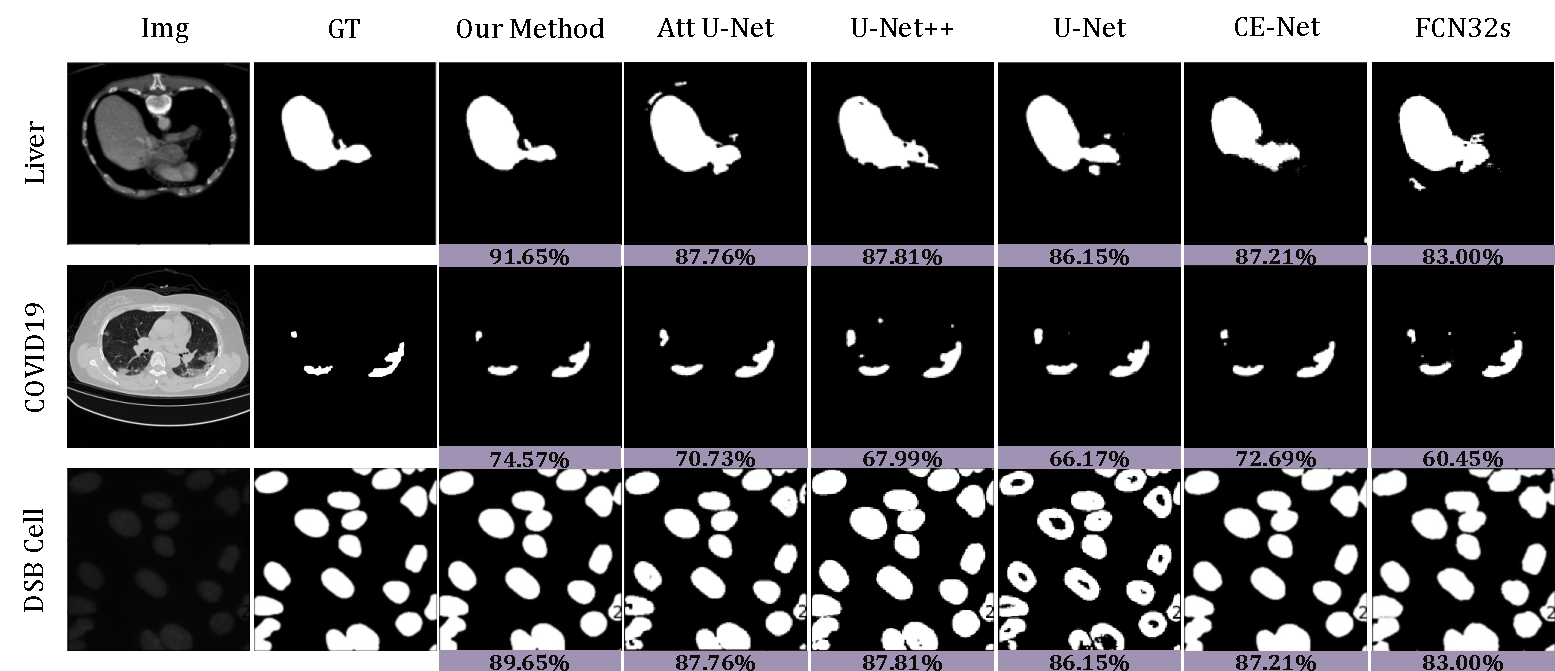
\includegraphics[width=0.99\textwidth]{figure/result.pdf}
  \vspace{-2mm}
  \caption{Medical image segmentation examples.} 
  \vspace{-2mm}
  \label{fig:result}
  \end{center}
  \vspace{-0.35cm}
\end{figure*}

我们利用U-Net,ResU-Net作为baseline,与我们提出的模型分别在Cell,Liver,COVID19三个数据集上进行对比
,每次实验所使用的参数,训练集,验证集,测试集均相同。
\subsubsection{Live segmentation results}
Segmentation results of cell segmentation are shown in tables \ref{dataset-table},在Dice. and F1 score指数上相比于
CE-Net, U-Net++, U-Net with Attention Gate, U-Net and FCN32s分别提升了1.30\(\%\), 1.49\(\%\), 4.35\(\%\), 6.11\(\%\) and 16.95\(\%\).
在Iou.指数上,分别提升了2.05, 2.27\(\%\), 6.08\(\%\), 7.30\(\%\) and 19.70\(\%\). 在Sens.指数上分别提升了9.80\(\%\), 6.53\(\%\), 7.39\(\%\), 
11.81\(\%\) and 15.36\(\%\). 在Hd.指数上分别降低了0.4074, 0.9083, 0.7471, 0.8825 and 2.4968.
  \begin{table*}[htbp]
    \vspace{-2mm}
    \begin{center}\small
    \label{dataset-table}
    \begin{tabular}{cccccccc}
      
    \toprule
    Datasets & Methods & Shape Loss & Dice. & F1 score. & Iou. & Sens. & Hd.\\
    \midrule
    \multirow{6}{*}{Cell} & Our proposal & $\surd$ & \textbf{0.8588} & \textbf{0.8588} & \textbf{0.7623} & \textbf{0.9296} & \textbf{4.6224}\\
                          & CENet & $\times$ & 0.8458 & 0.8458 & 0.7418 & 0.8316 & 5.2098\\
                          & UNet++ & $\times$ & 0.8439 & 0.8439 & 0.7396 & 0.8643 & 5.5307\\
                          & Attention UNet & $\times$ & 0.8153 & 0.8153 & 0.7015 & 0.8557 & 5.3695\\
                          & UNet  & $\times$  & 0.7977 & 0.7977 & 0.6893 & 0.8115 & 5.5049\\
                          & FCN32s & $\times$ & 0.6895 & 0.6895 & 0.5653 & 0.7760 & 7.1192\\
                          \hline
    \multirow{6}{*}{Liver}   & Our proposal & $\surd$ & \textbf{0.9551} & \textbf{0.9551} & \textbf{0.9165} & \textbf{0.9389} & \textbf{3.8854}\\
                          & U-Net++ & $\times$ & 0.9351 & 0.9351 & 0.8781 & 0.9156 & 5.8218\\
                          & Attention UNet & $\times$ & 0.9346 & 0.9346 & 0.8776 & 0.9056 & 4.836\\
                          & CENet & $\times$ & 0.9315 & 0.9315 & 0.8721 & 0.9045 & 4.904\\
                          & U-Net & $\times$ & 0.9253 & 0.9253 & 0.8615 & 0.9106 & 6.6785\\
                          & FCN32s & $\times$ & 0.9065 & 0.9065 & 0.8300 & 0.9381 & 7.97\\
                          \hline
    \multirow{6}{*}{COVID19} &  Our proposal & $\surd$ & \textbf{0.8489} & \textbf{0.8489} & \textbf{0.7457} & \textbf{0.8570} & \textbf{4.313}\\
                          &  CENet & $\times$ & 0.8348 & 0.8348 & 0.7290 & 0.9359 & 4.7711\\
                          &  UNet++ & $\times$ & 0.8014 & 0.8014 & 0.6799 & 0.9426 & 5.0301\\
                          &  Attention UNet & $\times$ & 0.8229 & 0.8229 & 0.7073 & 0.9435 & 4.8845\\
                          &  UNet  & $\times$ & 0.7874 & 0.7874 & 0.6617 & 0.9528 & 5.2231\\
                          &  FCN32s & $\times$ & 0.7409 & 0.7409 & 0.6045 & 0.9935 & 5.8644\\
  \bottomrule    
    \end{tabular}
    \caption{Comparsion With Other Methods In Cell\cite{dsb2018}, Liver\cite{liver} and COVID19\cite{covid19_2} Dataset}
  \end{center}
    %\vspace{-0.35cm}
    \vspace{-4mm}
  \end{table*}
\subsubsection{Cell segmentation results}
Segmentation results of cell segmentation are shown in table\ref{dataset-table}, 在Dice. and F1 score指数上相比于
CE-Net, U-Net++, U-Net with Attention Gate, U-Net and FCN32s分别提升了2.01\(\%\), 2.05\(\%\), 2.36\(\%\), 2.98\(\%\) and 4.86\(\%\).
在Iou.指数上,分别提升了3.84\(\%\), 3.89\(\%\), 4.44\(\%\), 5.50\(\%\) and 8.65\(\%\). 在Sens.指数上分别提升了2.33\(\%\), 3.33\(\%\), 3.44\(\%\), 
2.83\(\%\) and 0.08\(\%\). 在Hd.指数上分别降低了1.9362, 0.9506, 1.0186, 2.7931 and 4.0846.

  \subsubsection{COVID19 segmentation results}
  Segmentation results of covid19 segmentation are shown in table\ref{dataset-table}, 在Dice. and F1 score指数上相比于
  CE-Net, U-Net++, U-Net with Attention Gate, U-Net and FCN32s分别提升了1.41\(\%\), 4.75\(\%\), 2.60\(\%\), 6.15\(\%\) and 10.80\(\%\).
  在Iou.指数上,分别提升了1.67\(\%\), 6.58\(\%\), 3.84\(\%\), 8.40\(\%\) and 14.12\(\%\). %在Sens.指数上分别提升了2.33\(\%\), 3.33\(\%\), 3.44\(\%\), 2.83\(\%\) and 0.08\(\%\). 
  在Hd.指数上分别降低了0.4581, 0.7171, 0.5715, 0.9101 and 1.5514. 敏感度方面,通过观察Figure \ref{fig:result}我们可以发现
  ,其在分割目标图像时更加保守(改)。


  综上所述,我们的模型在三个数据集上均consistently outperforms CE-Net and U-Net with Attention-Gate. Figure \ref{fig:result}展示了我们
  在三个数据集上与其余5个模型的对比示例。COVID-19 ······, Liver ·······, Cell ·······。

  \section{Ablation study}
  To justify the effectiveness of the pretrained U-Net\cite{unet}, Res-UNet\cite{ResUNet}, 
  MRC(multi residual convolution) block, RMP block and SAR(spatial channel and gateway) Attention block
  in our proposed method, we conduct the following ablation study using the COVID19 and Cell dataset as examples.

  \subsection{Loss function}
  \begin{table*}[htbp]
    \vspace{-2mm}
    \begin{center}\small
        \label{loss-table}
        \begin{tabular}{ccccccc}
            \toprule
            Methods & Loss & Dice. & F1 score. & Iou. & Sens. & Hd.\\
            \midrule
            Our proposal & BCE          & 0.8076 & 0.8076 & 0.6874 & 0.8772 & 5.0112\\
            Our proposal & BCE+DiceLoss & 0.8375 & 0.8375 & 0.7282 & 0.8827 & 4.7241\\
            Our proposal & Ours         & 0.8489 & 0.8489 & 0.7457 & 0.8570 & 4.4313\\
        \bottomrule    
        \end{tabular}


        \caption{Comparsion With Other loss functions In COVID19\cite{covid19} Dataset}
    \end{center}
    \vspace{-4mm}
  \end{table*}
  为了验证我们使用的损失函数组合模型\(loss_{oveall}\)的有效性,我们以自己设计的模型作为baseline,在其他参数一致的情况下将其与\(loss_{BCE}\)和
  \(loss_{BCE+Dice}\)在COVID19数据集上进行对比,\(loss_{oveall}\)
  和\(loss_{BCE+Dice}\)的定义如下所示:
  \begin{align}
    loss_{oveall} = \alpha loss_{BCE} + \beta loss_{Dice} + \theta loss_{ACE}
  \end{align}
  \begin{align}
    loss_{BCE+Dice} = \alpha loss_{BCE} + \beta loss_{Dice}
  \end{align}
  在本次实验中,我们预先设置\(\alpha=0.5, \beta=0.5\)。对于\(\theta\),因为ACEloss与图像梯度有关,其loss value的范围通常为\([10^1, 10^5]\),所以\(\theta\)值应该
  显著小于\(\alpha, \beta\),在本次试验中,我们预先设置\(\theta=0.0005\)。实验结果如表\ref{loss-table}所示,对比于\(loss_{oveall}\)和\(loss_{BCE+Dice}\),在Dice.指标上
  我们分别提升了4.13\%, 1.14\%; 在F1 score.指标上我们分别提升了4.13\%, 1.14\%; 在Iou.指标上我们分别提升了5.83\%, 1.75\%; 在Sens.指标上我们分别降低了2.02\%, 2.57\%;
  在Hd.指标上我们分别降低了0.5799, 0.2928,其推理结果如图\ref{fig:ablation_loss}所示。
  \begin{figure}[htbp]
    \begin{center}
    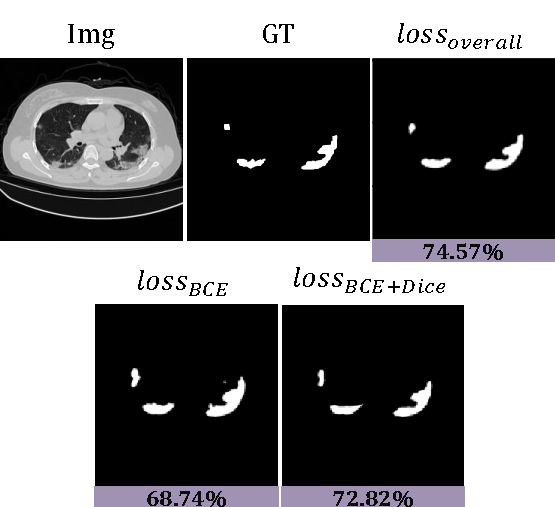
\includegraphics[width=0.45\textwidth]{figure/abliation_loss_img.pdf}
    \vspace{-2mm}
    \caption{不同损失函数训练下的模型推理结果} 
    \vspace{-2mm}
    \label{fig:ablation_loss}
    \end{center}
    \vspace{-0.35cm}
  \end{figure}




  \subsection{Modules}
  为了进一步验证我们设计的各个模块是否对分割任务有提升作用,我们将MRC Block, RMP Block, SRA Attention Block和shape loss function与ResU-Net分别进行组合:
  \begin{itemize}
      \item ResU-Net + MRC + RMP: to verify if this blocks can really 提升对深层图像特征的提取能力
      \item ResU-Net + SAR Attention Module: to verify if our Attention module can 更好地从spatial and channels角度enhanced pixel-wised segmentation than skip connection as well as
            attention-gate.
      \item ResU-Net + MRC + RMP +SAR: 分别使用\(loss_{BCE}\) and \(loss_{overall}\)来进行训练,用于验证组合模型的有效性。
  \end{itemize}

  \begin{table*}[htbp]
    \vspace{-2mm}
    \begin{center}\small
    \label{ablation-table}
    \begin{tabular}{cccccccc}
      
    \toprule
    Dataset & Methods & Loss & Dice. & F1 score. & Iou. & Sens. & Hd.\\
    \midrule
    \multirow{6}{*}{COVID19} & U-Net                & BCE  & 0.7874          & 0.7874          & 0.6617          & 0.9528          & 5.2231        \\
                             & ResU-Net             & BCE  & 0.8105          & 0.8105          & 0.6923          & 0.9601          & 5.0248        \\
                               & ResU-Net + MRC + RMP & BCE  & 0.8185          & 0.8185          & 0.7030          & 0.9295          & 4.8931        \\
                               & ResU-Net + SAR       & BCE  & 0.7988          & 0.7988          & 0.6846          & 0.7969          & 5.1522        \\  % trick
                               & ResU-Net+SAR+MRC+RMP & BCE  & 0.8076          & 0.8076          & 0.6874          & 0.8772          & 5.0112        \\
                               & ResU-Net+SAR+MRC+RMP & Ours & \textbf{0.8489} & \textbf{0.8489} & \textbf{0.7457} & \textbf{0.8570} & \textbf{4.313}\\
    \hline
    \multirow{6}{*}{Cell} & U-Net                & BCE & 0.7977 & 0.7977 & 0.6893 & 0.8115 & 5.5049\\
                               & ResU-Net             & BCE & 0.8314 & 0.8314 & 0.7274 & 0.9685 & 5.5861\\
                               & ResU-Net + MRC + RMP & BCE & 0.8448 & 0.8448 & 0.7414 & 0.9714 & 5.0647\\
                               & ResU-Net + SAR       & BCE & 0.8545 & 0.8545 & 0.7534 & 0.9669 & 4.9601\\
                               & ResU-Net+SAR+MRC+RMP & BCE & 0.8525 & 0.8525 & 0.7598 & 0.9744 & 4.9210\\
                               & ResU-Net+SAR+MRC+RMP & Ours & \textbf{0.8588} & \textbf{0.8588} & \textbf{0.7623} & \textbf{0.9296} & \textbf{4.6224}\\
  \bottomrule    
    \end{tabular}
    \caption{Ablation study for each component on COVID19 and Cell dataset}
  \end{center}
    %\vspace{-0.35cm}
    \vspace{-4mm}
  \end{table*}

  \paragraph{COVID19 ablation study result}
  我们将上述模型在COVID19数据集上进行测试并对比其IoU, F1 score, Dice, Sensitivity and Hd value. 每次实验所使用的参数,训练集,验证集,测试集均相同。
  如图\ref{fig:covid_comparison}和表\ref{ablation-table}所示:
  ResU-Net with MRC block and RMP block 对比于ResU-Net,Iou.指标提升了1.40\%, F1 score指标提升了1.34\%, Dice指标提升了1.34\%, Sensitivity指标提升了0.29\%, Hd指标降低了0.5214。
  ResU-Net with SRA attention module 对比于ResU-Net,Iou.指标提升了2.60\%, F1 score指标提升了2.31\%, Dice指标提升了2.31\%, Sensitivity指标降低了0.16\%, Hd指标降低了0.6260。
  \begin{figure}[htbp]
    \begin{center}
    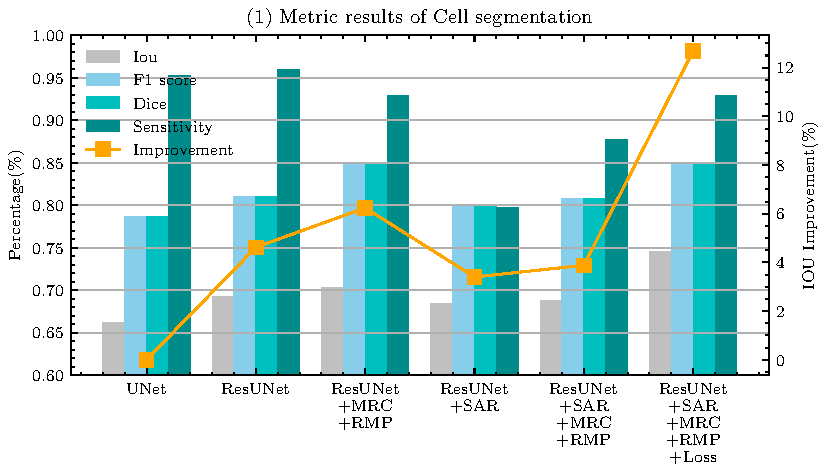
\includegraphics[width=0.45\textwidth]{figure/covid_comparison.pdf}
    \vspace{-2mm}
    \caption{Metric results of COVID19 segmentation compared with different models.} 
    \vspace{-2mm}
    \label{fig:covid_comparison}
    \end{center}
    \vspace{-0.35cm}
  \end{figure}
  ResU-Net with both SRA attention module and MRC, RMP module对比于ResU-Net,Iou.指标提升了3.24\%, F1 score指标提升了2.11\%, Dice指标提升了2.11\%, Sensitivity指标提升了0.59\%, Hd指标降低了0.6651。
  ResU-Net with both SRA attention module and MRC with the combination of shape loss function, 
  RMP module对比于ResU-Net,Iou.指标提升了3.49\%, F1 score指标提升了2.74\%, Dice指标提升了2.74\%, Sensitivity指标降低了3.89\%, Hd指标降低了0.9637。
  
  \paragraph{Cell ablation study result}
  我们将上述模型在Cell数据集上进行测试并对比其IoU, F1 score, Dice, Sensitivity and Hd value. 每次实验所使用的参数,训练集,验证集,测试集均相同。
  如图\ref{fig:cell_comparison}和表\ref{ablation-table}所示:
  ResU-Net with MRC block and RMP block 对比于ResU-Net,Iou.指标提升了1.40\%, F1 score指标提升了1.34\%, Dice指标提升了1.34\%, Sensitivity指标提升了0.29\%, Hd指标降低了0.5214。
  ResU-Net with SRA attention module 对比于ResU-Net,Iou.指标提升了2.60\%, F1 score指标提升了2.31\%, Dice指标提升了2.31\%, Sensitivity指标降低了0.16\%, Hd指标降低了0.6260。
  \begin{figure}[htbp]
    \begin{center}
    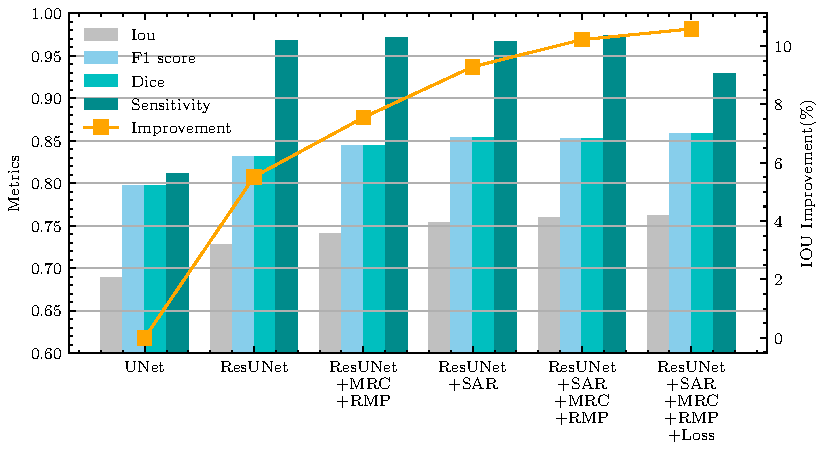
\includegraphics[width=0.45\textwidth]{figure/cell_comparison.pdf}
    \vspace{-2mm}
    \caption{Metric results of Cell segmentation compared with different models.} 
    \vspace{-2mm}
    \label{fig:cell_comparison}
    \end{center}
    \vspace{-0.35cm}
  \end{figure}
  ResU-Net with both SRA attention module and MRC, RMP module对比于ResU-Net,Iou.指标提升了3.24\%, F1 score指标提升了2.11\%, Dice指标提升了2.11\%, Sensitivity指标提升了0.59\%, Hd指标降低了0.6651。
  ResU-Net with both SRA attention module and MRC with the combination of shape loss function, 
  RMP module对比于ResU-Net,Iou.指标提升了3.49\%, F1 score指标提升了2.74\%, Dice指标提升了2.74\%, Sensitivity指标降低了3.89\%, Hd指标降低了0.9637。
  
  Furthermore, 通过将上述模型的IoU指标进行对比,我们可以发现相比于ResU-Net,both MRC+RMP module and SAR attention module 可以有效地提高模型的整体性能,同时两者的结合也能起到不错的提升效果(分别提升了
  1.84\%, 0.64\%)。同时,由于MRC block是CE-Net中DAC block的修改,所以我们也将该模型与CE-Net进行了对比,在IoU识别率仅仅降低了0.04\%的情况下,我们的模型实现了30.17\%的参数精简,提高了训练的速度和节省了模型的显存消耗。


\section{Conclusion}

\section{acknowledgment}

\bibliographystyle{IEEEtran}
\bibliography{complete.bib}

\begin{IEEEbiography}[{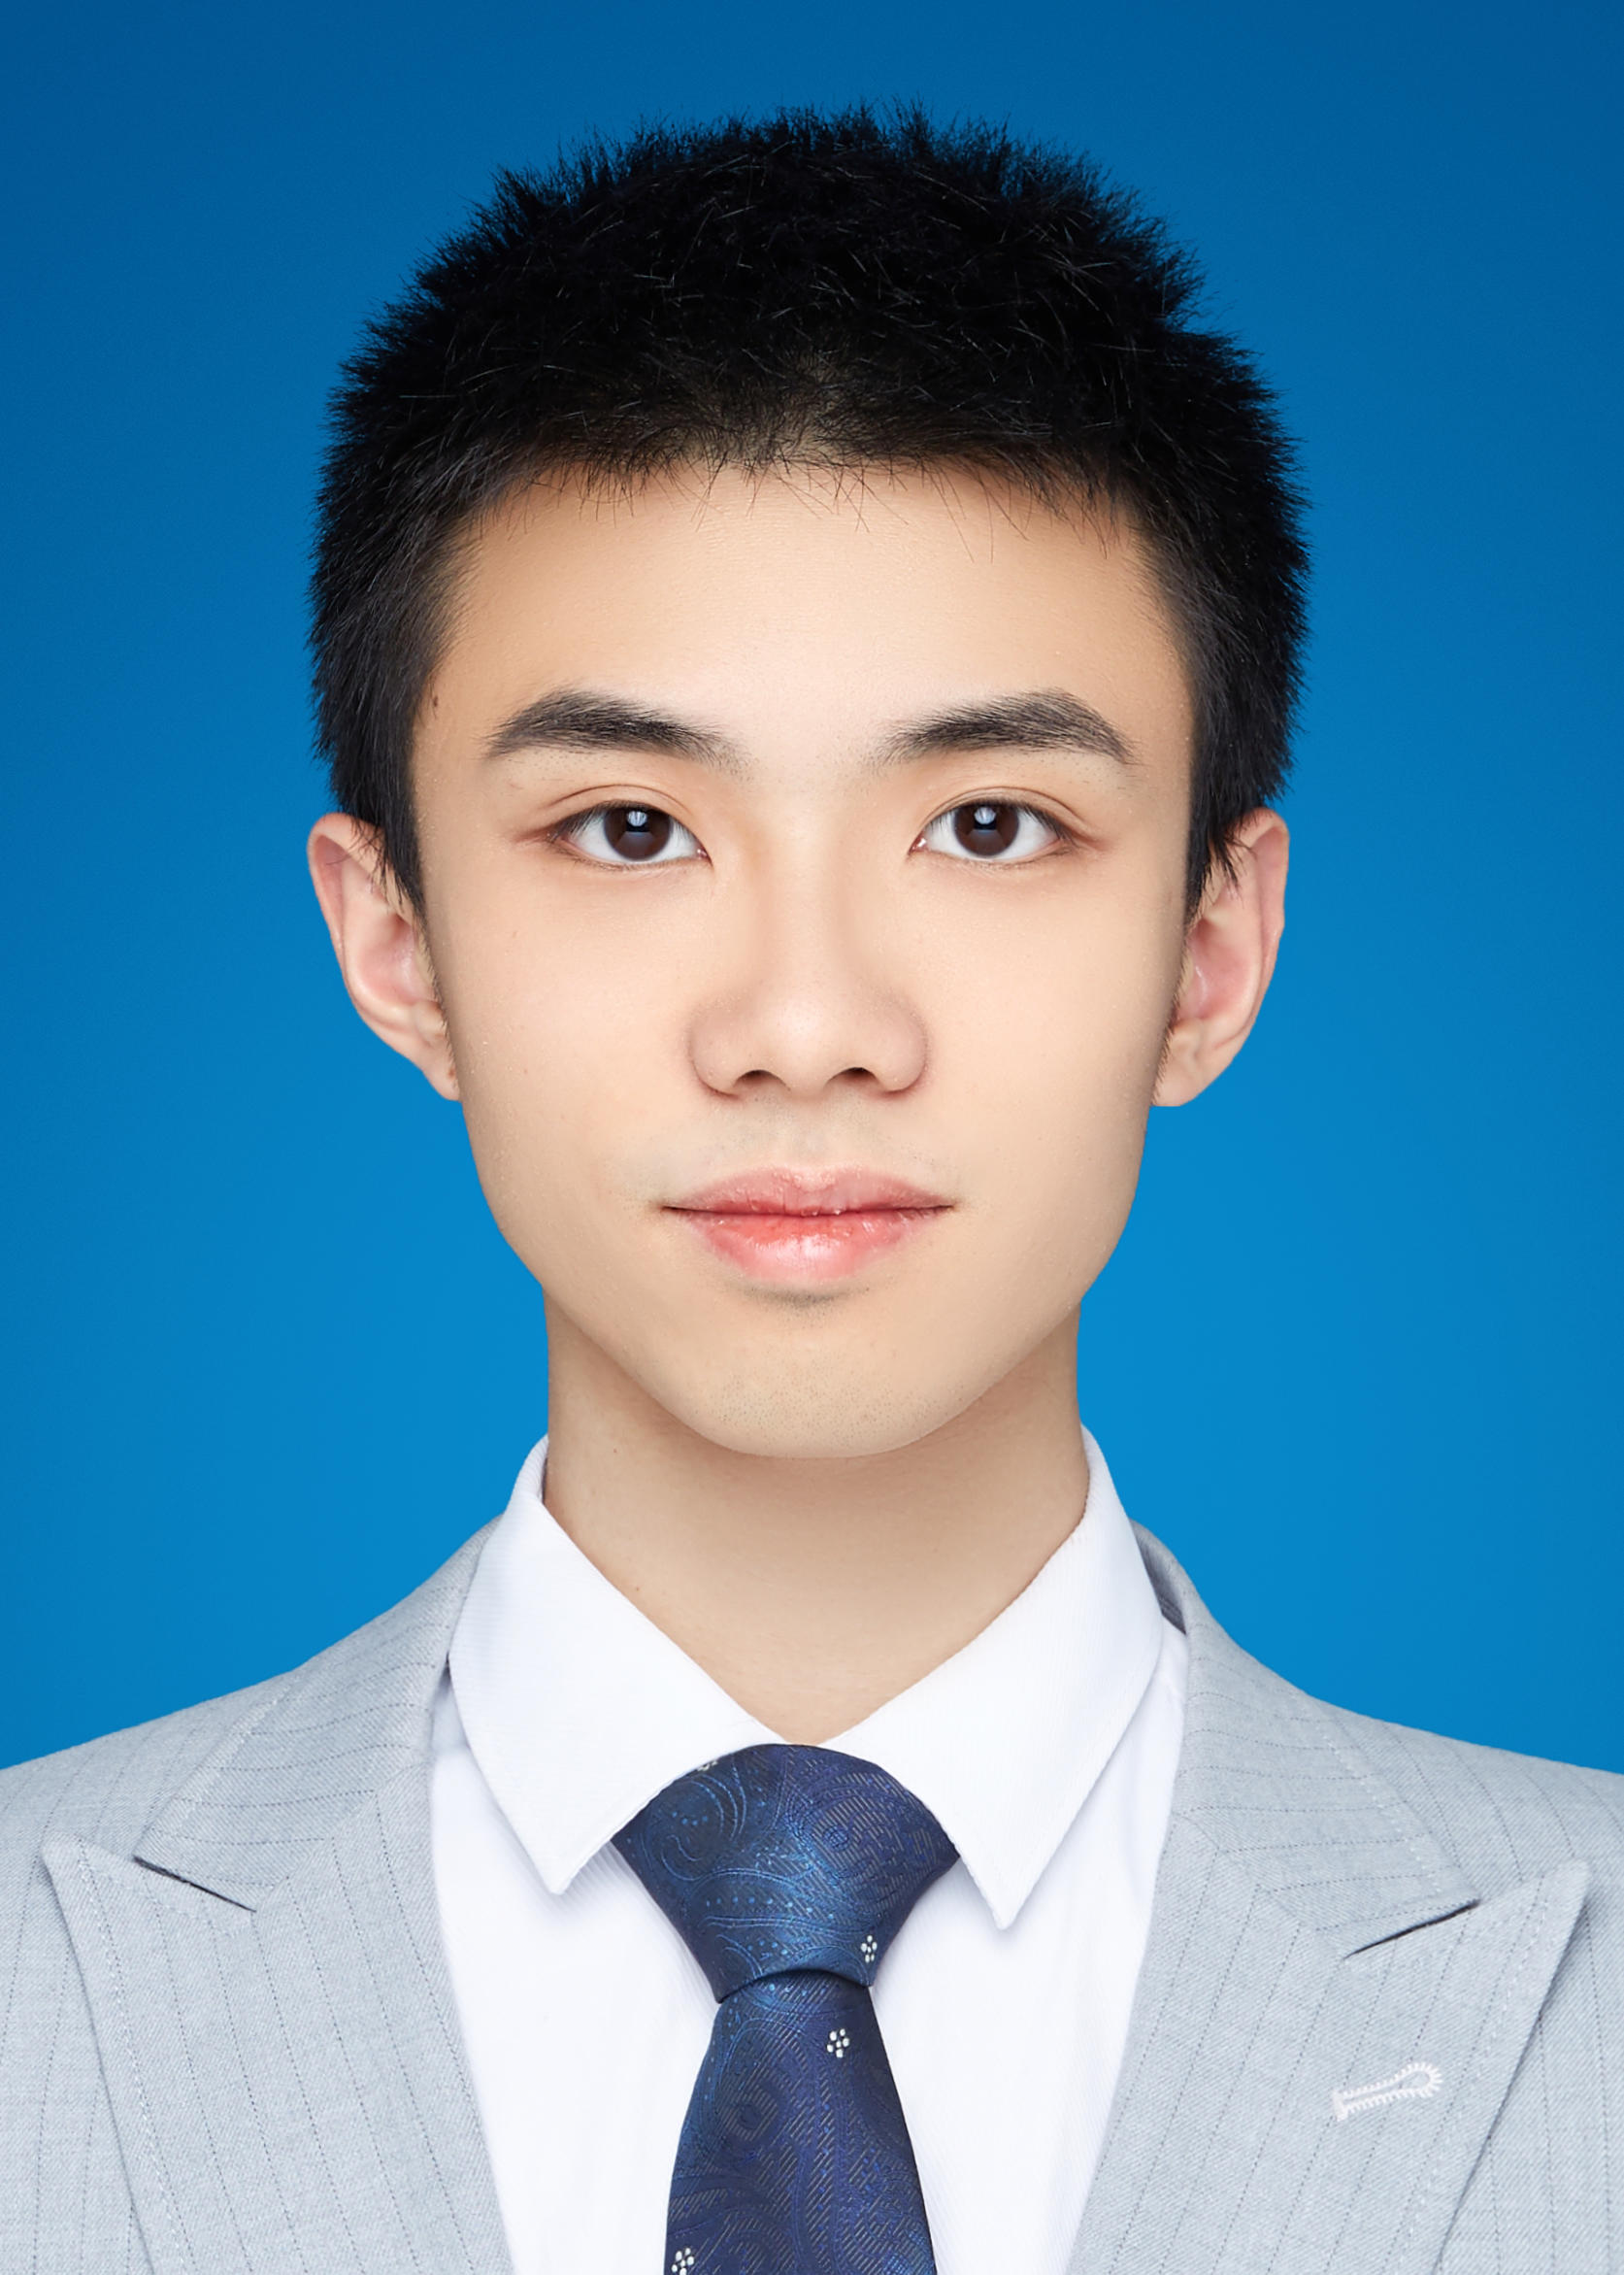
\includegraphics[width=1in,height=1.25in,clip,keepaspectratio]{lihao.png}}]{HAO LI} 
  is currently pursuing his bachelor's with the College of Information Science and Technology, Beijing University of Chemical Technology, Beijing.

  His research interest include robotics, computer vision and deep learning.
\end{IEEEbiography}

\begin{IEEEbiography}[{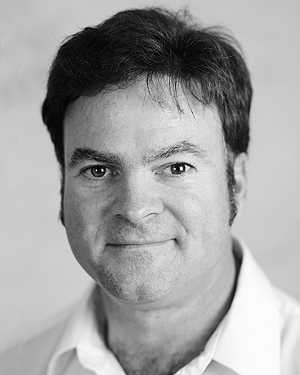
\includegraphics[width=1in,height=1.25in,clip,keepaspectratio]{a2.png}}]{Second B. Author} was born in Greenwich Village, New York, NY, USA in 
1977. He received the B.S. and M.S. degrees in aerospace engineering from 
the University of Virginia, Charlottesville, in 2001 and the Ph.D. degree in 
mechanical engineering from Drexel University, Philadelphia, PA, in 2008.

From 2001 to 2004, he was a Research Assistant with the Princeton Plasma 
Physics Laboratory. Since 2009, he has been an Assistant Professor with the 
Mechanical Engineering Department, Texas A{\&}M University, College Station. 
He is the author of three books, more than 150 articles, and more than 70 
inventions. His research interests include high-pressure and high-density 
nonthermal plasma discharge processes and applications, microscale plasma 
discharges, discharges in liquids, spectroscopic diagnostics, plasma 
propulsion, and innovation plasma applications. He is an Associate Editor of 
the journal \emph{Earth, Moon, Planets}, and holds two patents. 

Dr. Author was a recipient of the International Association of Geomagnetism 
and Aeronomy Young Scientist Award for Excellence in 2008, and the IEEE 
Electromagnetic Compatibility Society Best Symposium Paper Award in 2011. 
\end{IEEEbiography}


\EOD

\end{document}
